\documentclass[11pt,letter]{article}
\usepackage[top=1.00in, bottom=1.0in, left=1.1in, right=1.1in]{geometry}
\renewcommand{\baselinestretch}{1.1}
\usepackage{graphicx} %including pictrures 
\usepackage{natbib}
\usepackage{amsmath}
\usepackage{textcomp}
\usepackage[
singlelinecheck=false % <-- important
]{caption}
\usepackage{float}
\usepackage{hyperref}%helps with the email address 

\def\labelitemi{--}
\parindent=0pt

\def\labelitemi{--}
\parindent=0pt

\newenvironment{smitemize}{
\begin{itemize}
  \setlength{\itemsep}{0pt}
  \setlength{\parskip}{0.8pt}
  \setlength{\parsep}{0pt}}
{\end{itemize}
}

\graphicspath{ {./logPhotos/} }

\begin{document}
\bibliographystyle{/Users/Lizzie/Documents/EndnoteRelated/Bibtex/styles/besjournals}
\renewcommand{\refname}{\CHead{}}

\title{bcvin Fieldwork Log, May 2020}
\author{}
\maketitle
\tableofcontents

\subsection{4 May 2020}
\begin{smitemize}
\item Met with Pat Bowen and Carl Bogdanoff to discuss sampling and vineyard etiquette.
\item We should be allowed to leave up tape throughout the season and mark buds with metal tags but should ask first, of course
\item May be allowed to tag vines until next year for easy finding - ask managers
\item Pat and Carl don't think Arterra or Quail's Gate are doing organics management. Sebastian Farms is all organic now.
\item Merlot or Chardonnay would be good varieties to sample more throughly because they are commonly grown and popular for the region.
\item Slope aspect, east vs west side of lake (getting morning or afternoon sun), row direction - interests for climatic variation
\item the vineyard managers we are meeting should be considered more collaborators than facilitators. They might have good ideas.
\item to keep vine quality consistent, we should focus on vineyards directly managed by the big wine companies rather than contract growers. This is because contract growers get paid based on the amount of grapes they sell, rather than the quality of the grapes, so there is a tendency to overcrop. Mike may suggest a contract grower though that is growing to the higher standards, and if so we should go with his suggestion. As long as we keep to high quality vine management, the wine company should not make a big difference.
\item the most popular grape varieties shifts regularly. At the moment there is a lot of shifting to merlot from white winegrapes in the south. How it is probably 70:30 ratio of red to white there. More centrally in the valley it is more like 50:50. Sav blanc is getting more popular, and pinot gris is also popular at the moment
\item vines should be at least 4 years old for us to monitor them

\end{smitemize}

Grower communication
\begin{smitemize}
\item send growers information in easily digestible and usable formats i.e. simple spreadsheets or maps
\item make yourself useful by giving growers information that they want
\item Try never to say no to a talk or committee meeting invitation
\item Get on the Research and Development Council for BC Wine. Maybe attend conference if there is one.
\item when writing grants, deliverables must be useful.

\end{smitemize}

Need to consider: Make sure vines we choose will be there for 3 years
\vspace{1.5ex}

 We also briefly discussed winter hardiness modeling.
 \begin{smitemize}
\item Carl has started using a 4th order Quadratic equation, and this seems to be working well
\item acclimation and deacclimation are not the same process, but Carl thinks they should have similar rates
\item Carl also doesn't think there should be a relationship between maximum hardiness and rate of deacclimation. He pointed out Riesling bursts quite late, whereas Chardonnay bursts early, but they are both fairly hardy

\end{smitemize}

\subsection{5 May 2020}
\begin{smitemize}
\item met with Mike Watson at Dark Horse Vineyard, vineyard manager?/head viticulturist? at Arterra to discuss site access and what to consider when choosing vines
\item Mike is interested in soil type. Soil type can differ a within blocks, although less so for Arterra because Mike tries to avoid this issue. For contract growers, especially new growers, it is more of a problem because they focus on maximizing yield per hectare, so squish in as many vines as possible
\item Mike also mentioned something about a contract grower who "pushed the vines too much", who 3rd leaf on one year and second leaf the next, but mostly got away with it, although there were "circles of death" at the site. Mike seemed to think this might be related to the soil. He said some growers can get away with doing everything wrong, while others cant, and maybe this is because of soil. We didn't understand this section of the conversation.
\item some site maps might be incorrect, so Mike will send us updated maps
\item Fine to sample at Dark Horse, Whitetail, McIntrye, NK'MIP Cellars.
\item Dark Horse - We need to let Mike know we will be around. If we keep things non-onerous they can collect some data for us.
\item No expected variety/plant changes in the any of vineyards.
\item Flagging is fine, and we don't need signs as we don't want the workers to do anything special. We should use flagging tape that is not orange, yellow or pink though. (Faith also saw some blue while out at the vineyards).
\item Be aware that Inkameep Winery and NK'MIP Cellars are different. We are working at NK'MIP Cellars.
\item Phone numbers (to be contacted the day before entering the vineyard)
\item Manjit Deol (Manager at McIntrye and Whitetail) - 250 488 8215
\item Scott Carlson (Vineyard supervisor at McIntrye and WHitatail) - 250 485 7920. Call preferentially to Manjit because on site more
\item NK'MIP - Nelson Dutra (not sure of surname spelling) - 250 485 8085
\item there are also boards up at each vineyard with the spraying schedule. If in doubt, call Mike.
\item Call the day before to let vineyard know we will be sampling.
\item NK'MIP is usually locked, but we have a key. We should return the key at the end of the season.
\item we should access the vineyards between 6am and 3/4 pm. That is when the workers are there.
\item weekends should be ok. The workers work Saturdays but not Sundays though, so maybe we should avoid Sundays?
\item Nothing is alarmed
\item Mike talked very enthusiastically about a GIS dashboard they are working on that will have spraying schedules and stuff. Faith wonders if we could make our information (when we have it) a GIS dashboard, or a layer for their dashboard?
\item when we asked Mike what phenological stages he looks for, he mentioned "when the inflorescence separates". He uses this to gage what pesticides to use (whether to combine sulfur and pertritas or not). He's not sure how accurate this stage is, and we are not totally sure which Eichhorn - Lorenz stage it is, but we should try and capture it. It's a bit later than we would have thought to measure.

\end{smitemize}

Other notes from our Adventures:
\begin{smitemize}
\item why do Arterra cane prune rather than cordon prune some of the vines? Also we should consider how our flagging will work with these pruning types. Probably we need to use loose flagging so we don't restrict cane growth
\item Why do they spray irrigate in Whitetail? Also avoid rows where there are irrigation issues.
\item Mike has friends who rent Apex condos during summer if we can't find housing
\item Shiraz is Syrah! New revelation for Mira!
\item NK'MIP Cellars and McIntrye have Shiraz/Syrah
\item All 4 Arterra vineyards have Cabernet Sauvignon - consider adding to variety list

\end{smitemize}

Dark Horse Vineyard Walk notes
\begin{smitemize}
\item We should have 6 vines next to each other as a unit, and always skip to the first pole to avoid vines right on the outside edge of the block
\item We want probably a ratio of 40:40:20 of upper:lower:middle vines in the row. We also want to be as efficient with our time as possible, so avoid unnecessary crossing vine rows.
\item Sample near weather station
\item Merlot and Chardonnay are across the road from each other so make sampling plan easy to grab both.
\item Sample Merlot from several blocks and Chardonnay from both blocks

\end{smitemize}

NK'MIP Vineyard Walk notes
\begin{smitemize}
\item Sample both Merlot blocks, both Shiraz blocks, Cab Sau?
\item 6 top, 6 bottom, a few in middle

\end{smitemize}


\subsection{6 May 2020}

Chad meeting at Quail's Gate Wineshop to discuss Quail's Gate Estate Vineyard and Mannhardt Vineyard
\begin{smitemize}
\item Syrah/shiraz at Quail's Gate is not doing very well. 
\item In fact, very few of the vines below Boucherie Rd are doing very well. They are likely to be removed. Chad thinks this might be because the soil down there is more clay, whereas the top is more volcanic soil and gravel 
\item The Sauvignon blanc is ok though, probably there for 5 years.
\item Chad was not sure if there were good soil maps (we asked Pat and Carl and they said they have maps of soil)
\item Chad said we should sample in the other Quail's Gate vineyard (Mannhardt), where they have Riesling. 
\item Flagging tape is fine, and we don't need signs. We should label the flagging tape though with UBC and maybe Lizzie's name?
\item There are tags on every second row with vine rootstock, variety clone and block info. 
\item Chad doesn't think different blocks will be very different phenologically. 
\item There are weather stations on site
\item Chad was interested in the connection between numbers of flowers and numbers of fruit produced. Maybe we could capture this using software?
\item In passing, Chad mentioned there had been 90 per cent die off of buds. Not sure why, but I think from cold damage?
\item we could get pruning dates from Chad. He would be interested to see how pruning dates affect phenology. He talked about a trial where they tried to put back the phenology with late pruning. They did delay budbreak but then veraison was earlier. 
\item clone vs cordon pruning. Chad prefers cane pruning for high quality grapes because there is less chance of incorrect pruning leaving too many buds. He would be interested if pruning style affects phenology. The Riesling in Mannhardt would be good to try and tackle this question because there is a mix of pruning within the same block. But its possible vines might transition during our study.
\item Chad is trying to shift pruning so that a block is entirely cane or entirely cordon pruned. Some blocks are still mixed so pruning of some plants may change during experiment unless we flag them.
\item Rootstock 3309 is preferred because middle yield and good scion merging, 101/14 is good for lower vigour, and 504 is good for higher vigour. 
\end{smitemize}

Sampling
\begin{smitemize}
\item Chardonnay 4-1 is going to be changed, so don't sample. 3-4b is better. Don't sample 3-4a because it has a disease. Maybe utopia or something?
\item Blocks 5-1 to 5-4 are fine. 
\item management is fairly consistent in the vineyard. Apparently there are a few differences though. For example some of the Pinot noir clones are better than others so are either managed for quality or quantity, 4-11 and 3-1 are high quality. Other blocks not so high quality. For Chardonnay the top blocks 5-1 to 5-3 are less high quality and lower blocks 5-2 to 5-4. This is due to a spring in the top plus soil differences. Also perhaps a different clone?
\item But there are some trials of heat treatment instead of pertitiside. Tanya is doing this and may have phenology data. It would be interesting to see if differences based on this, but the current trials are on vines that will not stay. Chad would like to try on Pinot noir, and if so maybe we could get data from the different trials. 
 \end{smitemize}  

Access
\begin{smitemize}
\item We should text Chad, or even better Judy the Assistant Manager
\item No preferences on timing access or weekend vs weekday visits. 6 am is fine. Workers finish about 3.30pm.
\item There is a carpark opposite block 3-4a we can park in (just before the main shop, on the other side, if you are driving north from Penticton)
\item walking access is fine. Car access seems fine in Mannhardt but not Quail's Gate main vineyard. 
\end{smitemize}

\subsubsection {Meeting with Carl, Lizzie and Faith 2.30 pm}
\begin{smitemize}
\item generally we talked about winter hardiness (see CarlMeeting2020 document in hardiness folder)
\item Carl also supported what Chad said about popular rootstocks
\item we should be careful about s=rattle snakes 
\item we should get an exiting GIS Dashboard 
\item Carl was less convinced about the benefits of cane pruning, but talked about the difficulties of getting good pruning staff.
\end{smitemize}

\subsubsection{Meeting with Lizzie, Mira, Faith - sampling planning}
\begin{smitemize}
\item 300 plants in a variety rich plot at Davis took 4-6 hours to sample when interns got used to sampling. There was little walking between plants.
\item Save 20\% time to add Sebastian Farms sampling next year
\item Aim to sample 6 plants next to each other, do not go below 4 plants
\item Drop plants per block or diversity of locations within block before dropping diversity of blocks and varieties. No less than 16 plants per block.
\item Keep multiple blocks of a variety if they have the same rootstock and clone. If there are differences, it's less important to keep multiple blocks.
\item If desperate to lower numbers, look for variety overlap between McIntyre and Whitetail. 
\item If needed, order of dropping varieties = 1. Riesling, 2. Cabernet sauvignon, 3. Syrah. Not dropping: Sauvignon blanc, Pinot noir, Chardonnay, or Merlot.
\item Pick same rootstock if possible to minimize rootstock effect (S04?)
\item Plan for Dark Horse sampling to take about 1-1.5 hours so we can ask them to continue sampling after we leave.
\item Definitely try to do Brix sampling so we can compare with Mike's Brix
\item Try to prepare some report for Dark Horse as a thank you for helping us sample.

\end{smitemize}

\subsection{7 May 2020}
\begin{smitemize}
\item Flagged in Whitetail: 36 plants in block J Riesling, 36 plants in Chardonnay block OIB, 36 plants in Riesling block B, 24 plants in Chardonnay block C, 36 plants in Sauvignon blanc block D, 36 plants in Cabernet sauvignon block F.
\item Flagged in McIntyre: 24 in Cabernet sauvignon block Q, 36 in Pinot noir block O.
\item Merlot was not tagged in Whitetail because they were in the process of removing some vines and planting new ones. Will check for update next time we go to Whitetail.
\item Flags in Whitetail OIB likely to be removed
\item Scott Carlson gave us a key for McIntyre (and maybe Whitetail gates) so we can stay late if needed.
\item Initially used old orange flagging tape that we were drawing stripes on until last 12 plants of block D. Then began using new tape from Lizzie.
\item If cordon and cane, we chose to flag the cane.
\item If both cordons (or canes) looked fairly similar, we selected which cordon (or cane) to use by flipping a coin. Direction of heads and tails decided at beginning of block - consistent when blocks are same orientation.
\item GPS points were taken at each stop with the following naming formula: (2 letter vineyard code) - (block)(row\#)(location in row). Mira most often chose to use the even numbered row when naming but some may have the odd number. The even number was chosen because Mira likes even numbers.
\item An observation is that we saw a heard of horses grazing within the vineyard here. Is this for a land management reason, or an agreement between land owners/horse owners? DO the horses graze there all year? DO they damage or help (fertilize) the vines? 
\item We noticed in block C, there was quite a bit of within block phenological variation. Northern plants of row 30 were bursting bud or 2 leaves, and at the south end of the same row there were 3/4 leaves out
We saw a weather data logger at Whitetail 
\item McIntyre is on a bench/plateau overlooking the western side of the Okanagan Valley. You can just see the tail end of the lake from some places.
\item we saw what we think are fans in both McIntyre and Whitetail vineyards 
\item Mira noted there were totally different weed communities around the two vineyards. Might this suggest different soil types? We also saw what we think is evidence of fertilization, blue green pellets in the soil.
\item Lizzie suggested we think about buying a cheap printer, or asking Carl and Pat to print. Worst case Lizzie will post us some. 

\subsubsection {schedule}

\item 7.15 left Penticton 
\item 8.00 Arrived at Whitetail. 
\item We drove from lower vineyard to upper vineyard by following the road past OIB block. The road slopes up the side of the hill. 
\item 8.10 Walked up to block J .
\item Set up block J sampling.
\item 9.15 Left upper fields. 
\item 9.30 Drove through block middle of OIB. 
\item We set up 36 vines in block OIB and 36 in block B.
\item 11.18 Finished setting up blocks OIB and block B, and started driving to block C. 
\item 11.30 set up 24 vines in block C Chardonnay. 
\item We then went to Sav B. We noticed some vines have overhead and drip irrigation, where as others had only overhead 
\item 12.20 to 1.20 lunch break, and Lizzie visiting.
\item 13.23  drive to block B Sav B to finish last 12 vines.
\item 13.30 finished last 12 vine set up. 
\item 14.15 we headed to Merlot block G. Many plants here were too young. Also rows 55 plus were old but had lots of ripped up vines. we didn't end up setting anything up here yet.
\item 14.30 We popped over to the big metal shed where we met Scot (we think) and he gave us keys to McIntyre. We need to return the key at the end of the 3 weeks. 
\item 14.40 we went back to the vineyard and set 36 vines up at block F Cab Sav.
\item 15.08 left Whitetail for McIntyre vineyard.
\item 15.20 arrived McIntyre.
\item 15.30 sat and though about stuff and took photos.
\item 15.33 drove around to block Q and set 12 vines up.
\item 15.48 drove around.
\item 15.53 started setting more vines in block Q.
\item 16.04 finished setting the extra vines.
\item 16.07 drove to Pinot noir block O.
\item Block O has a mix of cordon and cane training vines. 
\item 16.28 finished the setting 24 vines in block O.
\item 16.33 Stopped at the other end of block O Pinot noir to set up last 12 vines close to the road.
\item 16.41 Finished setting up vines and went home.
\item 17.30 Arrived back in Penticton.

\end{smitemize}


\subsection{8 May 2020}
\begin{smitemize}
\item there are two road access points for McIntyre. The second (back entrance) is on Arrow Head Rd (off McKinney Rd, after main entrance) between block A and C.
\item Met Brian at NK'MIP while he was regulating irrigation. He drives around in a black truck and was nice enough to turn off the sprinklers in the row we were in without us asking.
\item Chad sent Mira contact information for Judy (Quail's Gate assistant manager)
\item 5.41am left Penticton .
\item 6.28am Arrived at McIntyre
\item 6.34 saw a deer in the vineyard.
\item 6.35 Set up block J Sav B. 12 vines many vines in.
\item Phenology vines ranged from green tips to leaves.
\item 6.46 drove to a new location (same block). Here we noticed there was a different clone for Sav B, and that around 75\% was the other clone. So we realised we needed to remove the 12 we had done that were clone 95 and replace them with clone 76. 
\item 6.57 finished checking clone info.
\item 7.09 set up 12 vines 6 vines in..
\item Phenology 1-4 leaves (E-L 7-11). 
\item 7.25 we heard that sprinklers would be in use for the next few hours in the other McIntyre blocks we wanted so we drove around the site to check layout and then left. 
\item 7.55 Arrived NK'MIP Cellars, and left car in carpark.
\item 8.05 Started sampling Syrah block C
\item Lots of age variety in this block, lots of very young (milk carton) plants mixed with mature vines. Maybe there was a die-off event? 
\item Phenology green tips to 5 leaves, although mostly 3 to 4 leaves. (E-L 4-12, although mostly 9-11).
\item Faith also noticed fertilizer? pellets in the soil. 
\item Vines on the top of the hill looked further along phenologically than those at the bottom.
\item 8.40 Finished block C Syrah.
\item 8.43 Arrived at lower NK'MIP (on foot).
\item 8.45 we started on block G (merlot). 
\item The vines very far along top of the hill. Phenology 5/6 leaves and inflorescence really obvious. Shoots 20cm long. (E-L 12-13).
\item 9.05 set up bottom 12 vines of block G, and then walked up the line to set up the top 12 vines.
\item Lower block Phenology 3 or 4 leaves. Some only 1 leaf. (E-L 9-11, although some 7) 
\item Upper of block Phenology 1 to 4 leaves, with most 2 to 3 leaves. (E-L mostly 9, some 7-4).
\item Lots of vines had cordons cut off, the wound painted blue green, and then canes. Others were still cordon pruned. 
\item Phenology buds from green tips to 3. A lot of 1 to 2 leaves separated. (E-L 4-9. A lot of 7-9)
\item 9.41 Finished first 12 of block B Cab sav.
\item We saw lots of orange and pink tape tied on the the poles.
\item Mira suggested that the distance counting 6 vines is quite variable.
\item 9.45 Started bottom 12 vines. 
\item Phenology some woolly buds onwards. Mostly 2 to 3 leaves. (E-L 3 onwards, most 9).
\item 9.53 Walked to upper 12 vines of same row 
\item 9.54 started the top 12 vines 
\item Phenology The vine looked further on than the other vines we looked at in the block. General 4 leaves and a clear inflorescence. (E-L 11/12) 
\item 10.05 Finished those 12 vines.
\item 10.07 we started on Block F Syrah.
\item This was a very small block, we struggled to fit even 24 sampling vines in. 
\item Phenology the vines were quite far on. 6 leaves plus inflorescence and shoots 20 to 30 cm long. Some only had 5 leaves. 
\item We needed a new role of tape here. 
\item 10.32 Finished Syrah block F.
\item 10.41 Left NK'MIP Cellars.
\item 11.10 Arrived Dark Horse. 
\item We had a break here 
\item 11.17 We were going to start block G, but we noticed the vines were on their own root stock. SO we went to look at block H as an alternative, but the plans were too young. SO we went back to block G. 
\item We set up bottom 12 vines here.
\item Phenology 2-3 leaves open, some had only 1 leaf and there were a few buds. (E-L some 1/2-7, others 9)
\item 11.34 Finished these vines and walked down the line.
\item 11.38 Started next 12 vines at top of line. 
\item One of the vies had canes that crossed over. We decided to use the direction of the end of the cane and ignore the crossover to chose which cane to sample. 
\item Phenology was diverse. from 1 leaf to 5 leaves. Most 2 to 3 leaves. (E-L 7-12)
\item 11.49 finished these vines. walked back down the row. 
\item 11.52 started middle 12 vines. 
\item Phenology same as in rest of block. 
\item 12.03 finished those vines. 
\item 12.05 walked to Chardonnay own root block B. Then we left.
\item 12.12 We tried to do the Merlot block B, but did not. 
\item This was because a nice man came on a quadbike to warn us that he had just sprayed sulfur there. We had had the all clear from Mike the day before, but had not double checked the spraying schedule. This was a mistake, always check the boards.
\item We then decided to leave and finish Dark Horse another day. 
\item 12.36 Arrived back in McIntyre.
\item Lunch break.
\item 12.57 Set block J Chardonnay middle row.
\item Phenology 3 to 4 leaves. (E-L 9-11) 
\item We noted that this block had south and north facing slopes in it.
\item 13.06 finished setting up the vines 
\item 13.12 removed the mistaken row we set up first thing in the morning.
\item 13.22 set 12 vines on the other side of block J (drove there).
\item Phenology mainly 2 to 3 leaves, with some 1 leaves and green tip buds. (E-L mostly 9, some 4-7)  
\item 13.47 Moved to block C (Riesling?), and started setting up 12 vines.
\item Phenology mostly green tips to 2 leaves. (E-L 4-7)
\item 14.00 Finished and walked up the line to the other end to set up the bottom 12 vines. 
\item 14.10 walk to middle 12 vines. 
\item We saw lost of baby vines (milk cartons) in this block. 
\item 14.14 start setting up middle 12 vines.
\item Phenology woolly buds to 2 leaves. (E-L 3-7)
\item 14.22 Finished and walked to the car.
\item 14.27 started block A.
\item Phenology woolly buds to 1 leaf. (E-L 3-7)
\item 14.44 Finished. Walked along and then down another row to do 12 middle vines. 
\item 14.54 finished. Walked back to car and drove to next vines.
\item 15.00 left the car.
\item The vines at the top seemed further along phenologically. green tips to 2 leaves. Maybe because this bit was on top south facing, whereas the bit we looked at before was in a sort of dip.
\item 15.08 finished those 12 vines. 
\item 15.13 moved to block E Sav B
\item Phenology generally green tip buds to 2 leaves. (E-L 3-7)
\item 15.21 Moved to middle of row.
\item 15.24 Did 12 vines.
\item 15.35 Drove around the block, and did the bottom 12 vines.
\item 15.45 Left vineyard.
\item 16.30 Arrived at Penticton.
\item After a break we typed up notes and chose blocks for Quails' Gate vineyards.
\end{smitemize}

\subsection{9 May 2020}
\begin{figure}%this will always show at this point 
  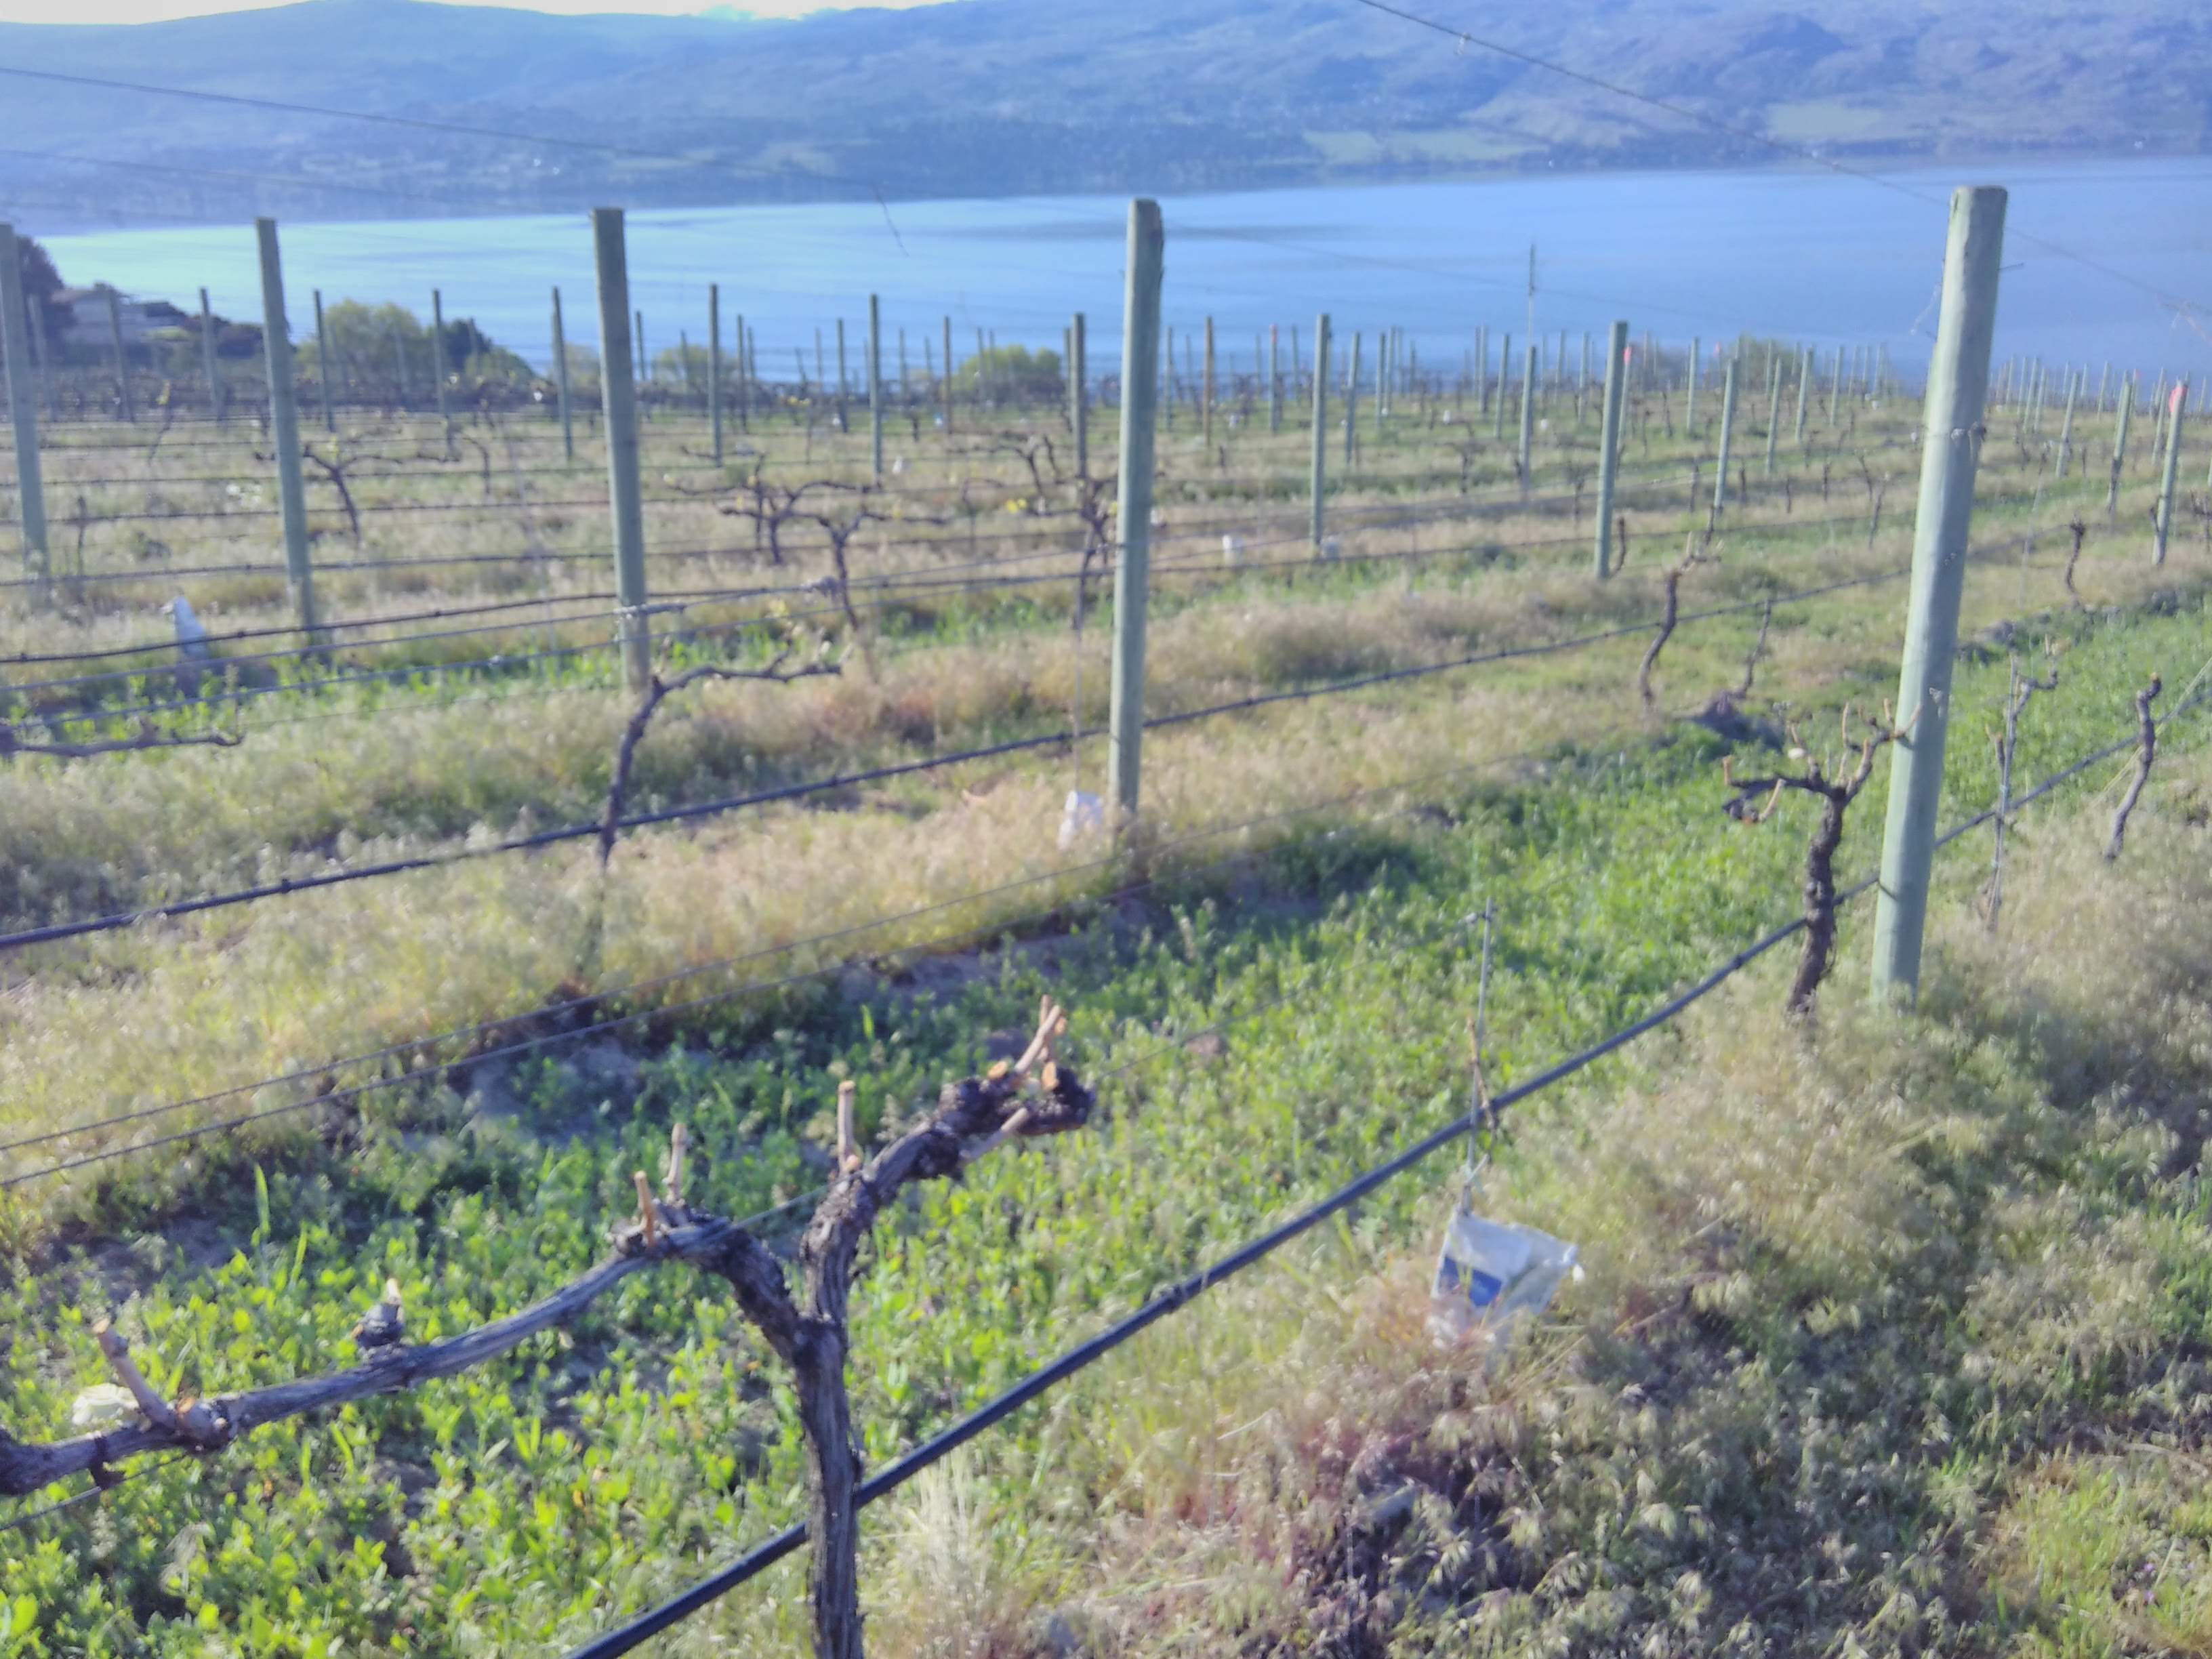
\includegraphics[width=\linewidth]{SyrahQGB1-2.jpg}
  \caption{There were lots of young vines in this Syrah block (QG 2-1) }
  \label{fig:SyrahSparse}
\end{figure}
\begin{figure}%this will always show at this point 
  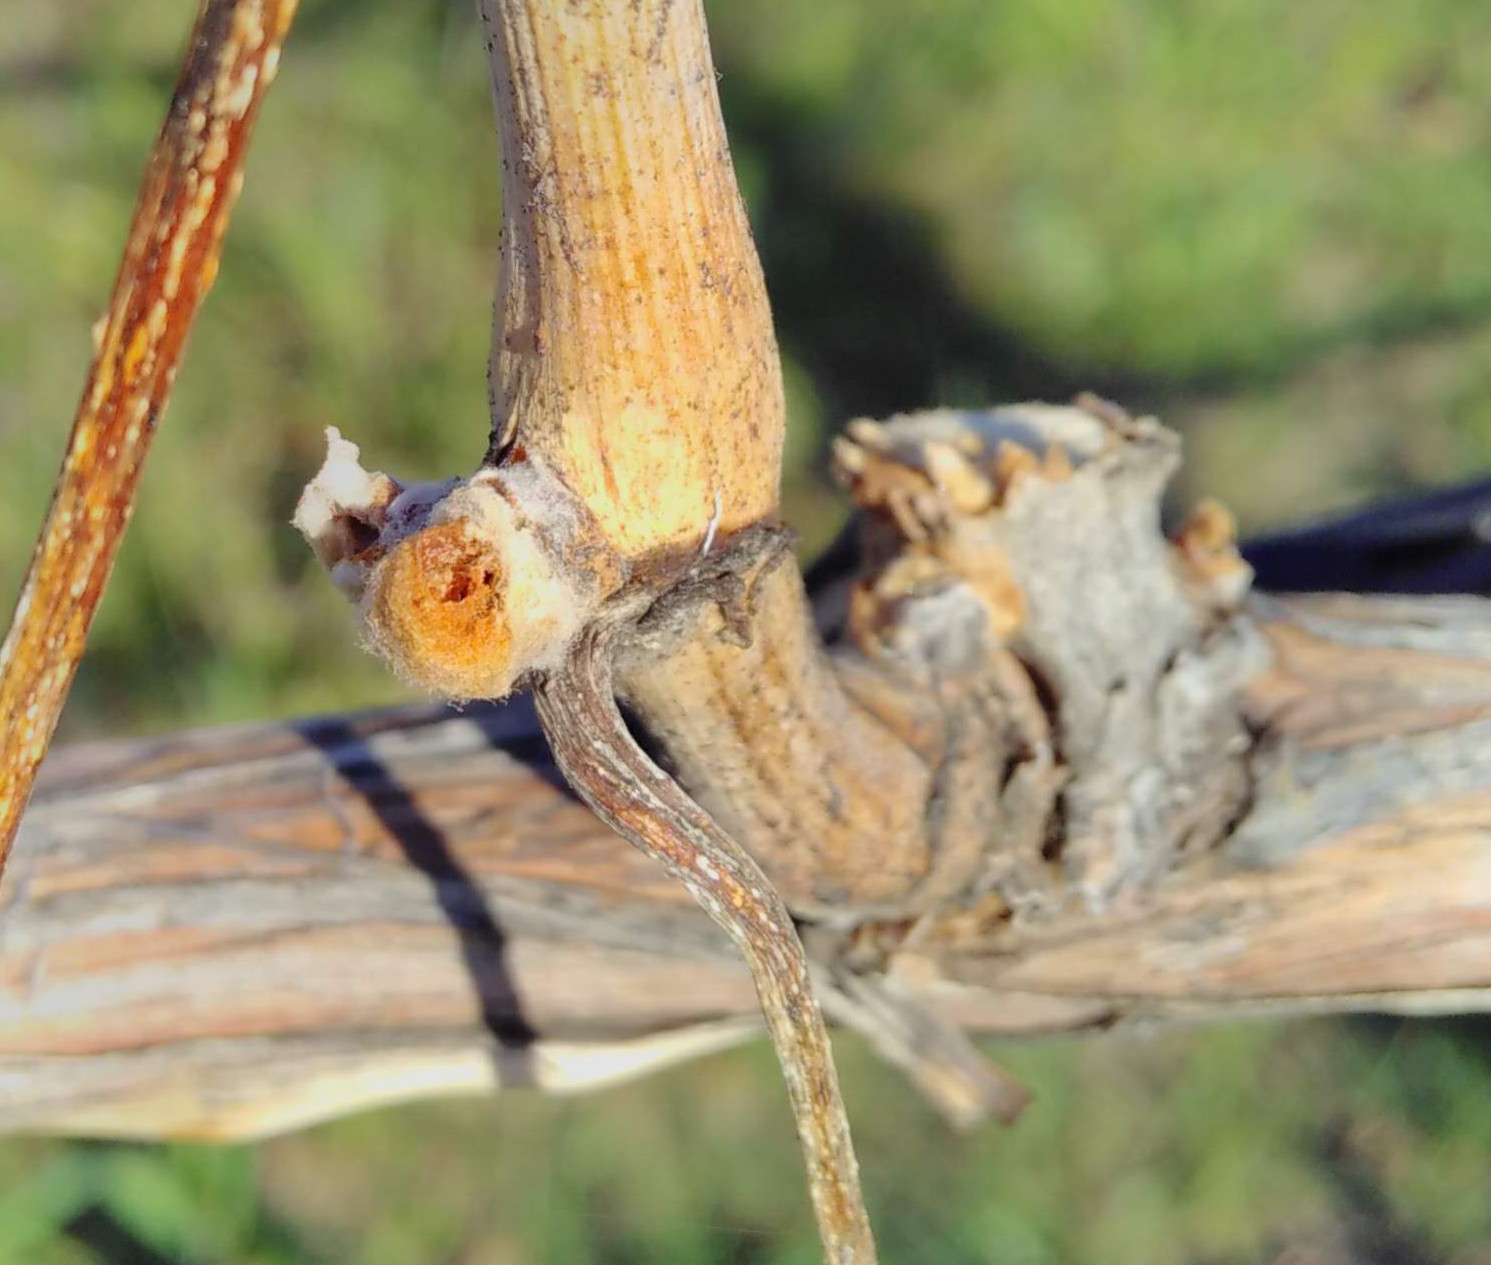
\includegraphics[width=\linewidth]{CutwormDamageSyrahQGB1-2.jpg}
  \caption{A bud in Quail's Gate Syrah block 2-1 that we think was damaged by cutworm }
  \label{fig:SyrahCutworm}
\end{figure}
\begin{smitemize}
\item 5.45 Left Penticton 
\item 6.46 Arrived at Quails' Gate main vineyard staff carpark, where we left the car.
\item 7.00 Arrived by foot at the lower part of the Quails' Gate vineyard, closer to the lake. We started at block 6 Sav B.
\item The signs are not great at this vineyard. The are laminated white pieces of paper, and many are missing or damaged. We mostly had to look at the signs at each corner of the blocks with QR codes, but these don't have row numbers.
\item Quite a few vines in this block only had one or cordon or cane. 
\item Phenology E-L 3-7.{}
\item These vines were on quite a steep south facing slope.  
\item 7.17 Finished those 12 vines.
\item 7.19 We moved onto the middle 12 vines. 
\item Phenology E-L 5-9.
\item 7.28 Finished these 12 vines and waled down the row to bottom 12 vines. 
\item 7.31 Started to bottom 12 vines.
\item We had to skip quite a few vines because they did not have enough spurs with buds. 
\item 7.44 Finished those vines and walked to the Syrah block 2-1.
\item The Syrah block had a lot of young plants in amongst the older vines. It took us awhile to find 12 vines that had enough older vines. This problem was especially bad in the West end of the block (Figure \ref{fig:SyrahSparse}).
\item we think we saw a cutworm damaged bud, see Figure \ref{fig:SyrahCutworm}. 
\item 8.00 Finished those 12 vines, and walked down the row. 
\item Faith noticed the portable washrooms are locked. We should ask if we can get the code. 
\item Faith lost her phone and then found it again.
\item 8.24 Finished the lower 12 vines and walked around to the middle 12 vines. 
\item Phenology E-L 1-7.
\item This block goes almost right to the cliff at edge of the lake. 
\item Above this point there were lots of missing vines. 
\item 8.35 Walked back to car. 
\item 8.45 Back to the car, and then from there into the upper vineyard. 
\item we changed the batteries in the GPS. 
\item 9.03 Arrived at Chardonnay block 5-4
\item Here we saw 2 plants with cutworm damage on them. One only had a single damaged bud that we saw, whereas another one had lost most buds.
\item Phenology E-L 3-9. 
\item 9.13 Finished these 12 vines, and walked up the row.
\item This is a really long block with a path through the middle.
\item 9.19 Arrived at the top of this block to do the top 12 vines.
\item some buds looked damaged.
\item Phenology E-L 1-7. Most 3-4. 
\item 9.33 Finished these vines and walked to next block.
\item 9.37 Started Merlot block 6-1. 
\item Phenology mostly 4-5. 
\item These buds were really pink. 
\item 9.46 Finished those 12 vines and walked to the top of the row.
\item Phenology E-L 3-5.
\item 9.55 Finished those vines and walked to the middle of the row. 
\item 10.00 We did the middle 12 vines.      
\item Phenology 1-5. Mostly 3 and 4. 
\item 10.09 Finished these vines and walked to block 4-8 Pinot noir
\item On the way we noticed a weather station near the bottom of Merlot block 6-2.  
\item 10.15 We did the top 12 vines of block 4-8 Pinot noir. 
\item Phenology E-L 1-9. 
\item Canes seemed further along than cordons. 
\item 10.23 Finished these vines and walked down to do the bottom 12 vines. 
\item 10.26 Reached the bottom of the row to set up the bottom 12 vines. 
\item Phenology E-L 1-9. Most 4-5, and pinkish.
\item 10.33 Finished these 12 vines, and started walking to the car. 
\item 10.45 Reached the car and had a break.  
\item 10.50 Walked to the Pinot noir block 3-3.
\item Phenology E-L 1-3. Mostly 1. 
\item 10.59 Finished those 12 vines and walked to upper 12.
\item 11.01 Started the upper 12 vines.
\item Phenology E-M mostly 1-2.
\item 10.10 Finished those vines. 
\item We saw a lot of mourning doves and American robins at Quails' Gate in general. 
\item 11.14 We went to Sav blanc block 4-6 and started upper 12 vines. 
\item Phenology E-M 3-7.
\item 11.25 Finished these vines and walked to the top of the row. 
\item 11.28 Set up the top 12 vines. 
\item Phenology E-L 4-9.
\item 11.37 Finished these vines and walked to the middle row 12 vines.
\item 11.39 Started on middle 12 vines.
\item Phenology E-M 5-7 
\item 11.46 Finished those vines and walked to Chardonnay block 3-4b.
\item 11.50 Started the top 12 vines. 
\item Phenology was a bit different for cordons and canes. 
\item Phenology (cordons) E-L 3-7 
\item Phenology (canes) E-L 7-9.
\item 11.58 Finished those vines, and walked down to the bottom of the row. 
\item 11.59 Started the lower 12 vines
\item Phenology same as above. 
\item 12.07 Finished those vines and walked to the car.
\item 12.10 Left for Mannhardt vineyard.  
\item 12.15. Had a lunch break.
\item While we were eating, a lady walked back and asked what we were doing. We had a nice chat, and then she told us about her father. It turns out she is the daughter of the man who set up the vineyard at Mannhardt, although it was an orchard first. Her name is Ines, and her father is Reiner. According to Ines, her father kept climate records for 40 years at that sites. She said we could try and email him (and cc her) to ask for it, but we should be aware that he is over 90 and had a few strokes so is not very fast. Her email is \href{mailto:ines.mannhardt@telus.net}{ines.mannhardt@telus.net}. Reiner's email is \href{mailto:reiner_mannhardt@telus.net}{reiner\_mannhardt@telus.net}.
\item 13.45 Finished lunch.  
\item This vineyard has much better signs
\item 12.56 Arrived by foot (we left the car near the gate) to Riesling block 8-6. 
\item There was quite a bit of cutworm damage 
\item Phenology E-M 3-7
\item 13.04 Finished 12 upper vines and walked down the block.
\item We decided not to set these 12 vines at the very bottom because there was a dip at the bottom of the block that looked like it might effect climate. As we were only sampling 24 vines we didn't want that much within block variation. 
\item 13.09 arrived at the middle/end of the block to set up the 12 vines
\item Phenology E-L mostly 3, some 5.
\item 13.15 Finished, and walked to next block. 
\item 13.18 Set up 12 vines in Pinot noir block 8-8. 
\item Phenology E-L mostly 7, some as early as 4. 
\item 13.26 Finished, and walked up the row. 
\item There seemed to be more grassy weeds here than the other vineyards. 
\item 13.26 Did the top 12 vines of this block.
\item Phenology E-L mostly 4-7. Some 3. 
\item 13.37 Finished and walked to Riesling block 9-1.
\item 13.44 Arrived at the top of Riesling block 9-1, and started setting up 12 vines. 
\item Phenology E-M mostly 4-5. 
\item 13.51 Finished those 12 vines, and walked sown the row. 
\item 13.52 Arrived at lower 12 vines. 
\item Phenology E-L 4-7. 
\item 13.58 Finished those 12 vines and walked up to the middle row for the last 12 vines. 
\item 14.00 set 12 vines 
\item Phenology E-L 4-7. 
\item 14.08 Finished and waled to the car. 
\item 14.12 Got to car to drive home.
\item 15.30 arrived home in Penticton. The roads were a lot busier this way, but not problematic. 
\item A break and then note writing. 
\end{smitemize}

\subsection{TO DO:}
\begin{smitemize}
\item Make "how to get where document" add links to Carl's maps on github
\item Seb Farms names - first 2 letters = variety, 3rd letter = block? Add block for each variety to the variety names document for Carl
\item add Judy contact info to repo
\item Maybe contact Mr Mannhardt 
\item Make a protocol 
\end{smitemize}

\end{document}